\documentclass{book} % Definisi jenis dokumen

%%%%% Definisi paket-paket yang seharusnya digunakan %%%%%
\usepackage[utf8]{inputenc} % paket encoding input utf8
\usepackage[T1]{fontenc} % paket encoding huruf latin
\usepackage{tocbibind} % paket toc terdaftar dalam toc

%%%%% Definisi paket-paket yang digunakan sesuai kebutuhan %%%%%
\usepackage[yyyymmdd,hhmmss]{datetime} % paket tanggal-waktu
\usepackage{geometry} % paket ukuran kertas dan margin
\usepackage{graphicx} % paket grafik/gambar
\usepackage{subcaption} % paket untuk subfigure

%%%%% Pengaturan ukuran kertas dan margin %%%%%
\geometry{
    a4paper,
    left=10mm,
    right=10mm,
    top=15mm,
    bottom=15mm,
}

%%%%% Pengaturan perintah informasi perangkat lunak (hanya untuk GNU/Linux) %%%%%
\newcommand{\ShowOsVersion}{
    \immediate\write18{\unexpanded{foo=`uname -sro` && echo "${foo}" > tmp.tex}}
    \input{tmp}\immediate\write18{rm tmp.tex}
}

\newcommand{\ShowTexVersion}{
    \immediate\write18{\unexpanded{foo=`pdflatex -version | head -n1 | cut -d' ' -f1,2` && echo "${foo}" > tmp.tex}}
    \input{tmp}\immediate\write18{rm tmp.tex}
}

\begin{document}

    %%%%%%%%%%%%%%%%%%%%%%%%%%%%%%%%%%%%%%%%%%%%%%%%%%%%%%%%%%%%%%%%%

    \frontmatter % untuk halaman cover

    \begin{titlepage}

        \centering % untuk membuat tengah teks

        {
            \LARGE % pakai font besar
            \bf % pakai font BOLD
            Rangkuman Improvement Prototype P2 dan P3
        }

        \bigskip
        {\Large \bf Achmadi ST MT}
        \vfill % menambahkan ruang kosong vertikal

        
\includegraphics[width=300pt]{images/elbicare-logo}
        \vfill

        \raggedright
        \noindent Dokumen ini ditulis dengan:\\ % tanda \\ menambahkan garis baru
        OS : \ShowOsVersion \\
        TeX : \ShowTexVersion \\
        Update: {\today} at \currenttime\\
    \end{titlepage}

	%%%%%%%%%%%%%%%%%%%%%%%%%%%%%%%%%%%%%%%%%%%%%%%%%%%%%%%%%%%%%%%%%
	
	\newpage % halaman baru
	\tableofcontents % daftar isi
	\listoffigures % daftar gambar
	\listoftables % daftar table

    %%%%%%%%%%%%%%%%%%%%%%%%%%%%%%%%%%%%%%%%%%%%%%%%%%%%%%%%%%%%%%%%%
    
    \mainmatter % pindah format halaman dari romawi ke angka (konten utama)
    
    \newpage
    \chapter{Definisi}
    
    Berikut beberapa definisi umum yang digunakan dalam dokumen ini:
    
    \begin{enumerate}
    	\item \textbf{P2}: Mengacu pada desain Prototype Versi 2 yang 
    	dikembangkan selama awal tahun 2021 sebagai acuan awal desain produk
    	
    	\begin{figure}[!ht]
    		\centering
    		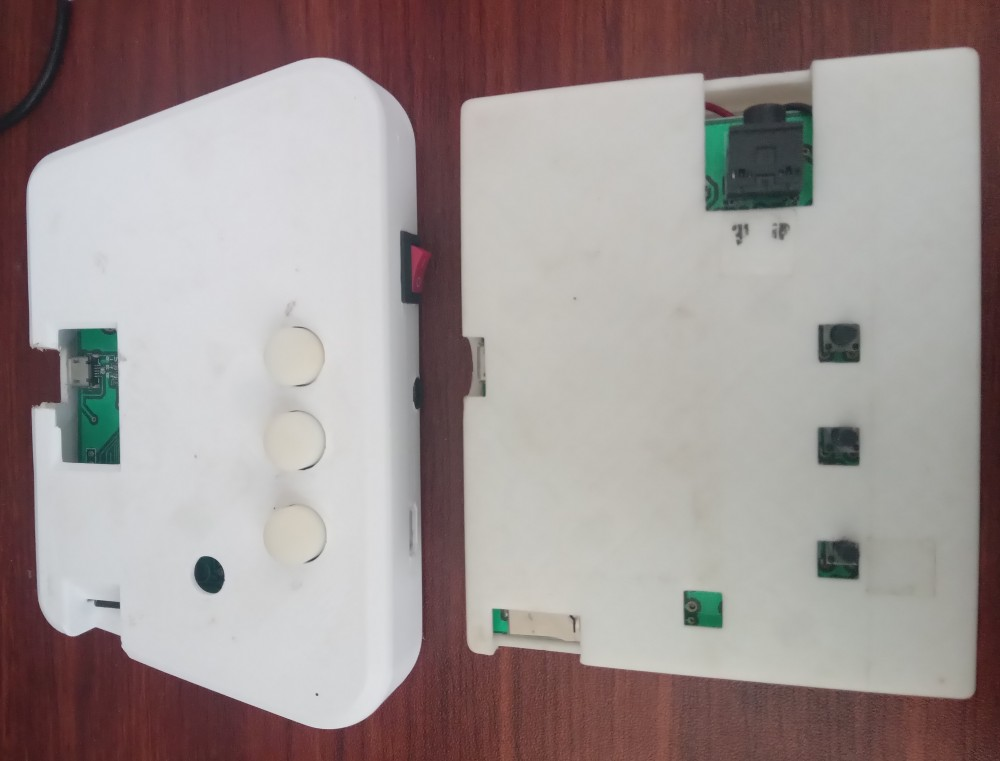
\includegraphics[width=300pt]{images/p2}
    		\caption{Gambaran Unit P2 (kanan) dan Unit P2 dengan improvisasi 
    		casing (kiri)}
    	\end{figure}
    
    	\item \textbf{P3}: Mengacu pada desain Prototype Versi 3 yang 
    	dikembangkan sejak akhir tahun 2021 sebagai desain produk siap produksi 
    	massal
    	
    	\begin{figure}[!ht]
    		\centering
    		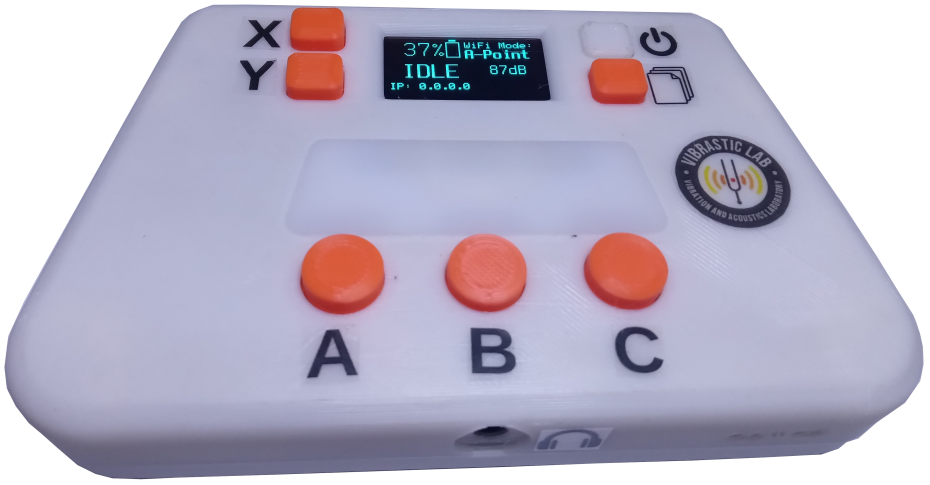
\includegraphics[width=300pt]{images/p3}
    		\caption{Gambaran Unit P3}
    	\end{figure}
    \end{enumerate}
    
    \newpage
    \chapter{Circuit}
    
    Berikut dirangkum perbaikan produk di aspek desain sirkuit elektronik 
    tercetak (PCB), yang dibagi dalam grup-grup komponen.
    
    \section{STM32}
    
    Untuk penggunaan chip utama Audiometri, yaitu STM32 ARM Cortex-M4, tidak 
    mengalami perubahan jauh.
    
    \begin{figure}[!ht]
    	\centering
    	\begin{subfigure}[t]{0.25\textwidth}
    		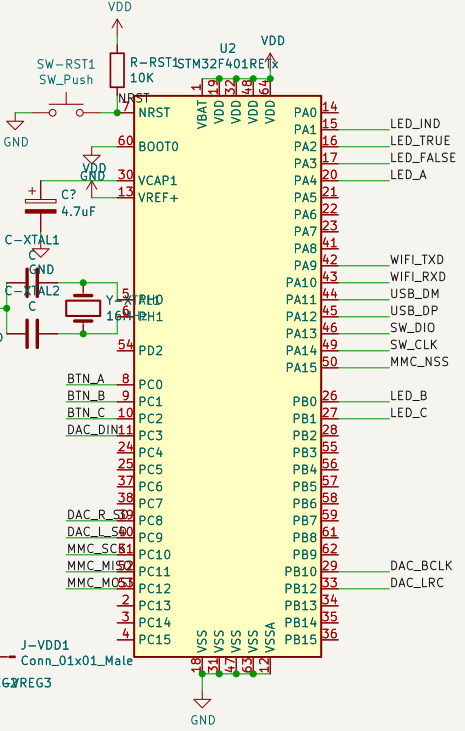
\includegraphics[width=\textwidth]{images/p2_stm32}
    		\caption{STM32 pada P2}
    	\end{subfigure}
    	\begin{subfigure}[t]{0.40\textwidth}
    		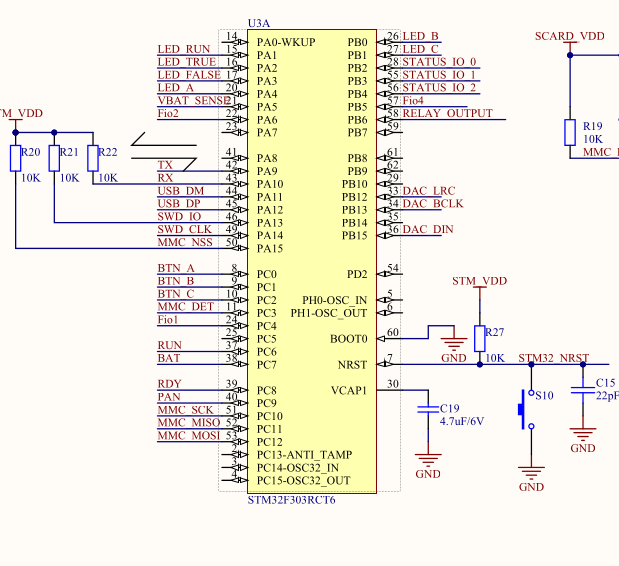
\includegraphics[width=\textwidth]{images/p3_stm32}
    		\caption{STM32 pada P3}
    	\end{subfigure}
    	\caption{STM32 sebagai chip Audiometri}
    \end{figure}

	Beberapa poin rangkuman perbaikan:
	\begin{itemize}
		\item Kompatibel dengan chip STM32 ARM Cortex-M4 untuk paket LQFP64.
		Chip yang telah digunakan adalah STM32F401RET6 dan STM32F303RBT6
		
		\item External RC/Crystal source dihapus
		
		\item Tambahan pull-up resistor pada beberapa pin.
		Beberapa catatan terkait pull-up resistor untuk desain selanjutnya:
		\begin{itemize}
			\item SWD-IO tidak boleh ada pull-up
			\item Pull pada USB-DM harus dipindah ke USB-DP
		\end{itemize}
	\end{itemize}

	Chip STM32 Cortex-M4 ini yang menangani proses \textit{3-Force Choice} (3FC) ,
	pembuatan sinyal PCM untuk nada murni, serta olah data hasil Audiometri via USB-Serial.
    
    \section{ESP32}
    
    Penambahan modul ESP32 (ESP-WROOM-32) adalah fitur baru yang sebelumnya 
    tidak ada pada P2.
    Modul ini ditambahkan sebagai penunjang antar muka pengguna dalam penggunaan 
    Audiometri yang ditangani oleh chip STM32
    
    \begin{figure}[!ht]
    	\centering
    	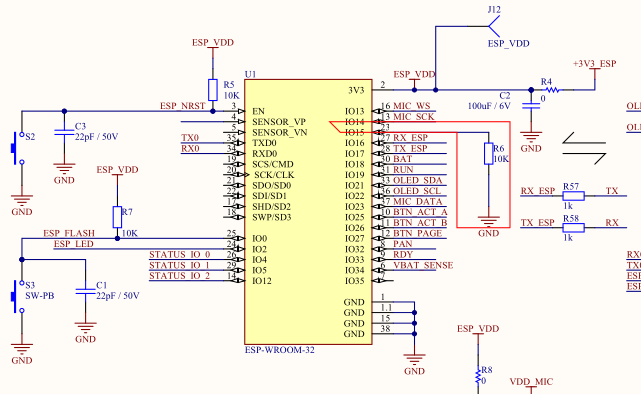
\includegraphics[width=400pt]{images/p3_esp32}
    	\caption{Modul ESP32 pada P3}
    \end{figure}
	
	\newpage
	Fitur yang akan ditangani oleh modul ESP32 meliputi:
	\begin{itemize}
		\item \textit{Drawing} untuk tampilan layar dan data ke pengguna
		\item Komunikasi data dengan server untuk wadah data pengguna via WiFi Station
		\item Pengaturan unit via WiFi Access Point
		\item Memantau besar derau audio lingkungan
		\item Memantau status fitur-fitur pada unit
	\end{itemize}
    
    \section{Power}
    
    Untuk bagian pengaturan daya, telah mengalami perbaikan sangat signifikan sehingga desain P3 menjadi lebih stabil.
    
    \begin{figure}[!ht]
    	\centering
    	\begin{subfigure}[t]{0.25\textwidth}
    		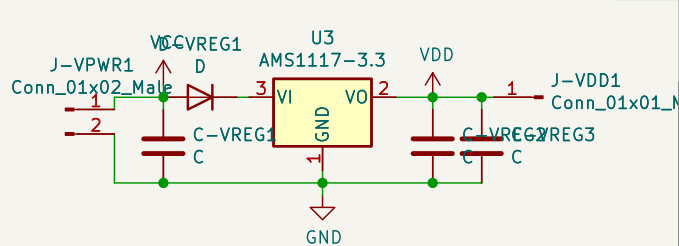
\includegraphics[width=\textwidth]{images/p2_vreg}
    		\caption{Power Regulator pada P2}
    	\end{subfigure}
    	\begin{subfigure}[t]{0.40\textwidth}
    		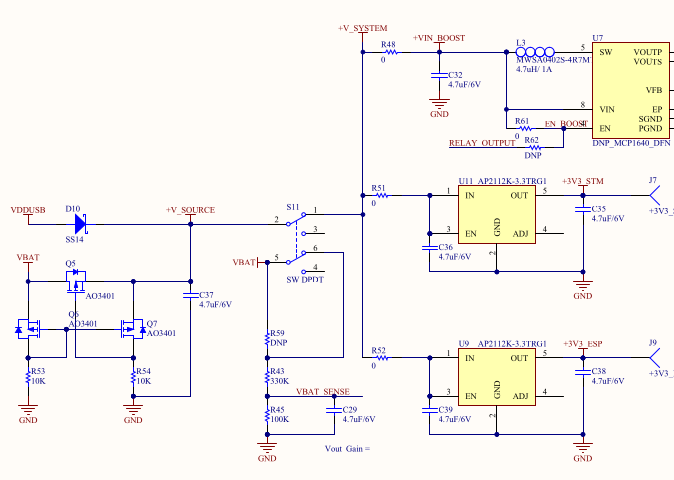
\includegraphics[width=\textwidth]{images/p3_vreg}
    		\caption{Power Regulator pada P3}
    	\end{subfigure}
    	\caption{Power Regulator}
    \end{figure}

	Beberapa poin rangkuman perbaikan antara lain:
	\begin{itemize}
		\item Regulator utama diganti dari berbasis AMS1117 LDO 3v3 menjadi AP2112K 3v3.
		\item Pemisahan regulator daya menjadi beberapa grup sesuai kebutuhan
	\end{itemize}
    
    \section{Audio DAC}
    
    Untuk bagian Audio yang menghasilkan nada murni, chip yang digunakan tetap MAX98357A.
    Namun mendapat perubahan desain terkait pengaturan channel kiri dan kanan.
    
    \begin{figure}[!ht]
    	\centering
    	\begin{subfigure}[t]{0.25\textwidth}
    		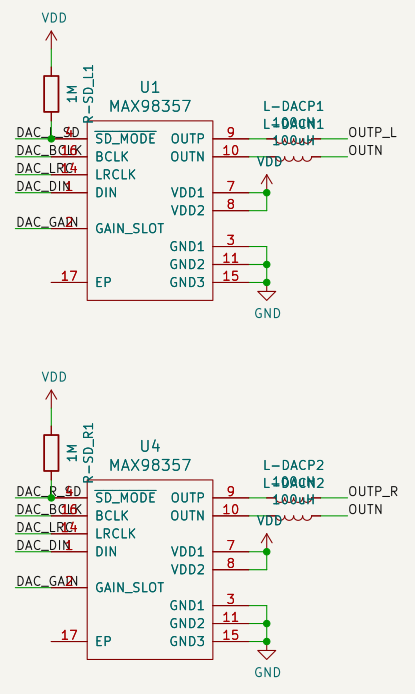
\includegraphics[width=\textwidth]{images/p2_dac}
    		\caption{Audio DAC pada P2}
    	\end{subfigure}
    	\begin{subfigure}[t]{0.60\textwidth}
    		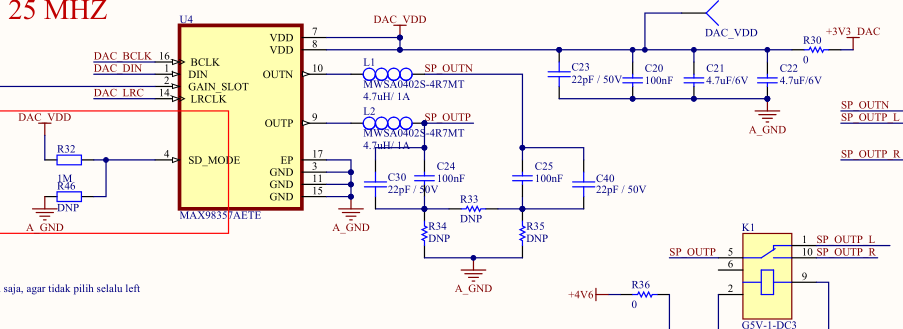
\includegraphics[width=\textwidth]{images/p3_dac}
    		\caption{Audio DAC pada P3}
    	\end{subfigure}
    	\caption{Audio DAC}
    \end{figure}

	Beberapa poin rangkuman perbaikan antara lain:
	\begin{itemize}
		\item Audio DAC menggunakan relay sebagai pemisah channel, bukan lagi 2 chip tersendiri
		\item Tambahan banyak decoupling capacitor dan filter pada output
		\item Mendapat regulator tenaga tersendiri (terpisah dengan chip/modul utama lain)
	\end{itemize}
    
    \section{Display}
    
    P3 mendapat fitur baru berupa OLED LCD untuk membantu pengguna.
    OLED LCD yang digunakan berupa 128x64 LCD yang terhubung ke modul ESP32 melalui jalur I2C.
    
    \begin{figure}[!ht]
    	\centering
    	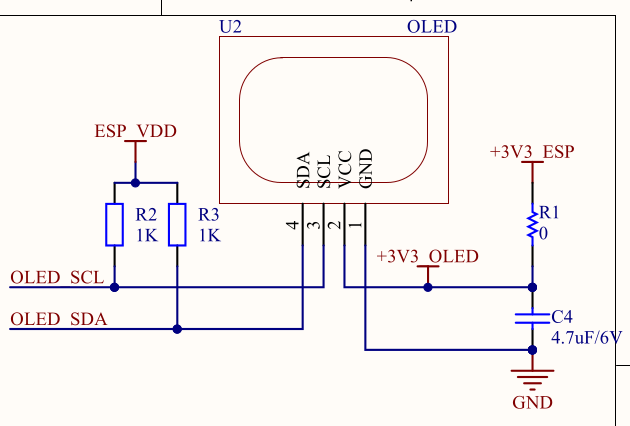
\includegraphics[width=300pt]{images/p3_oled}
    	\caption{Modul OLED LCD}
    \end{figure}
    
    \newpage
    \section{Storage}
    
    Untuk penyimpanan hasil Audiometri, baik P2 dan P3 sama-sama menggunakan MicroSD yang
    terhubung dengan STM32 melalui jalur SPI.
    
    \begin{figure}[!ht]
    	\centering
    	\begin{subfigure}[t]{0.25\textwidth}
    		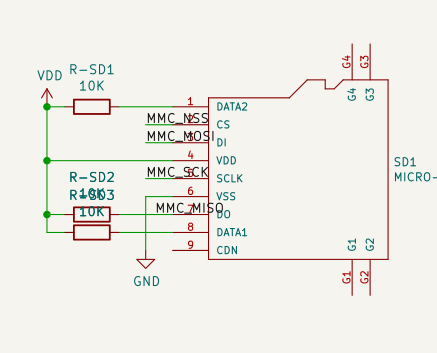
\includegraphics[width=\textwidth]{images/p2_mmc}
    		\caption{MMC pada P2}
    	\end{subfigure}
    	\begin{subfigure}[t]{0.60\textwidth}
    		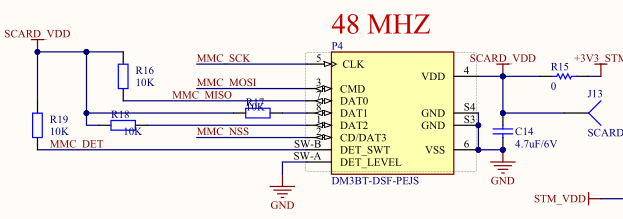
\includegraphics[width=\textwidth]{images/p3_mmc}
    		\caption{MMC pada P3}
    	\end{subfigure}
    	\caption{Slot MMC}
    \end{figure}

	Beberapa poin rangkuman perbaikan antara lain:
	\begin{itemize}
		\item Slot diganti ke pinout kompatibel DM3BT.
		\item Pin deteksi diaktifkan dengan tambahan pull-up resistor.
	\end{itemize}

	Catatan: Diperlukan beberapa purchasing komponen slot MMC yang kompatibel DM3BT.
    
    \section{USB-Data}
    
    \section{Microphone}
    
    \chapter{Casing}

\end{document}
